\section{Solution Description}

In order to handle graphs instead of linear input (strings), we modify Iguana according to~\cite{Grigorev:2017:CPQ:3166094.3166104}. We also provide the ability to switch between the SPPF construction and reachability facts calculation. It avoids unnecessary memory usage when the paths calculation is not required.

As far as the original GLL is aimed to handle arbitrary (even ambiguous) context-free grammars, our solution can handle arbitrary grammars too. It makes the solution less restrictive with regard to a query specification language, thus being more user-friendly.

\begin{figure}[ht]
    \centering
    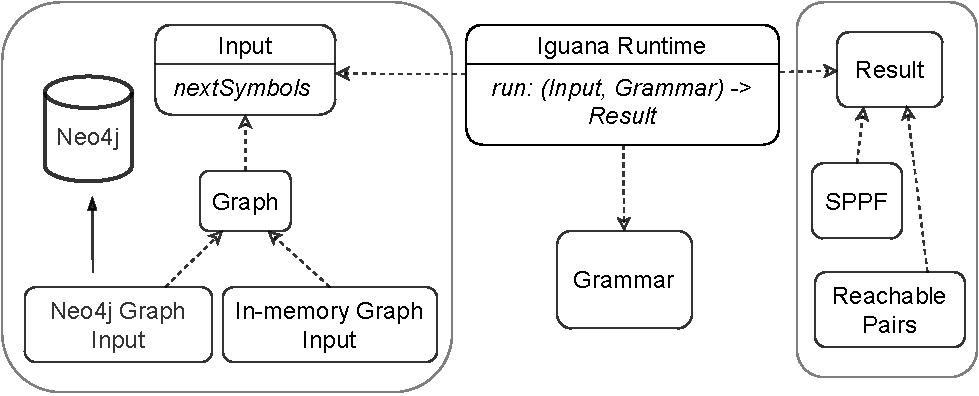
\includegraphics[width=0.47\textwidth]{architecture.pdf}
    \caption{Architecture of the solution}
    \label{fig:solution_architecture}
\end{figure}

The main parts of the solution are presented in figure~\ref{fig:solution_architecture}. \texttt{Iguana Runtime} takes an \texttt{Input} and a context-free \texttt{Grammar} to produce the \texttt{Result}. \texttt{Input} abstracts a data structure with the ability to get the next symbols for the given position. One example of \texttt{Input} is \texttt{Graph}, in which the position is a vertex, and the next symbols are the labels of its outgoing edges. We implement two different graphs. The first is a simple in-memory graph, and the second is a wrapper for Neo4j. Communication with the database is done using the Neo4j Native Java API. We used an embedded database, which means it is run inside of the application and is not used as an external service. Note that the architecture is extensible, and one can provide their own implementation of \texttt{Graph} to enable context-free path querying for a new graph storage.

Along with the existing modifications of GLL we made a Neo4j-specific one. Neo4j returns the outgoing edges of a vertex as a \texttt{Stream} and it is important to prevent early stream forcing, thus we chaged all GLL internals to ensure that. This also has an added benefit that the query result is a stream, and thus it is possible to get the results on demand. 

%Additionally, we add a switch that allows one does not create SPPF if only reachability information is needed. SPPF is needed only for paths reconstruction, so if one wants to get only reachable pairs, SPPF construction can be omitted, which leads to performance improvements and memory consumption decreasing.

The \textit{multiple sources} querying is natural for GLL as far as this algorithm is \textit{directed} as opposed to the naive linear algebra based algorithms. So, to support the multiple sources context-free path querying, we need only to be able to specify the start vertices for traversing, and no nontrivial modifications of GLL are required.  

